\providecommand{\qcor}[1]{\ulcorner#1\urcorner}   %
\providecommand{\qcOne}{\mathbf{1}}   %
\providecommand{\hK}{\hbar\mathcal{K}}   %
\providecommand{\hQCat}{\hbar\mathcal{Q}\mathrm{Cat}}   %
\providecommand{\evid}[1]{\mathrm{ev}_{\qcor{\mathrm{id}_{#1}}}}   %

\section{Yoneda 引理}\label{sec:yoneda-lemma}

设 $b\colon\qcOne\to B$ 是∞-范畴 $B$ 中的一个元素，并考虑其作为%
\trCommaInfinityCategory{}的右表示 $\mathrm{Hom}_{B}(B,b)$。
余定义域投影函子在此情形不提供额外的信息，但定义域投影函子
$p_{0}\colon\mathrm{Hom}_{B}(B,b)\twoheadrightarrow B$ 却具有一个由推论 5.5.14
所表达的特殊性质：它定义了一条\trDiscreteCartesianFibration。
由于这一映射在元素 $x\colon\qcOne\to B$ 之上的诸\trFiber{}是定义 3.4.9 的%
\trMappingSpace{} $\mathrm{Hom}_{B}(x,b)$，我们把
$p_{0}\colon\mathrm{Hom}_{B}(B,b)\twoheadrightarrow B$ 视为对由 $b$ 所表示的%
反变函子的编码。

本节的目标是在这一设定中陈述并证明\trYonedaLemma，其中诸反变可表示函子被编码为%
\trDiscreteCartesianFibration。
非正式地说，\trYonedaLemma{}断言：「在恒同处求值定义了一个等价」，而这里所说的
恒同元素是函子
\begin{center}
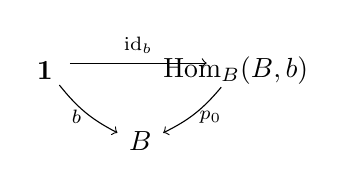
\begin{tikzpicture}[x=1.5em,y=1.5em]
  \node (o) at (0,0) {$\qcOne$};
  \node (H) at (4.6,0) {$\mathrm{Hom}_{B}(B,b)$};
  \node (B) at (2.3,-1.7) {$B$};
  \draw[->] (0.6,0.18) -- node[above]{$\scriptstyle\qcor{\mathrm{id}_{b}}$} (3.9,0.18);
  \draw[->] (0.35,-0.35) to[bend right=12] node[left,pos=0.6]{$\scriptstyle b$} (1.75,-1.5);
  \draw[->] (4.25,-0.4) to[bend left=12] node[right,pos=0.6]{$\scriptstyle p_{0}$} (2.85,-1.5);
\end{tikzpicture}
\end{center}
严格说来，$\qcor{\mathrm{id}_{b}}$ 并不生活在 $B$ 之上的切片∞-宇宙中，因为其
定义域对象 $b\colon\qcOne\to B$ 不是\trIsofibration；尽管如此，对任何%
\trIsofibration{} $p\colon E\twoheadrightarrow B$，沿 $\qcor{\mathrm{id}_{b}}$
的限制都会在切片拟范畴式\trFunctorSpace{}之间诱导出一个函子
\[
\mathrm{Fun}_{B}\bigl(\mathrm{Hom}_{B}(B,b)\xrightarrow{\ p_{0}\ }B,\,
E\xrightarrow{\ p\ }B\bigr)
\xrightarrow{\ \mathrm{ev}_{\qcor{\mathrm{id}_{b}}}\ }
\mathrm{Fun}_{B}\bigl(\qcOne\xrightarrow{\ b\ }B,\,
E\xrightarrow{\ p\ }B\bigr)
\]
这里其余定义域是由如下\trPullback{}定义的\trQuasiCategory：
\begin{center}
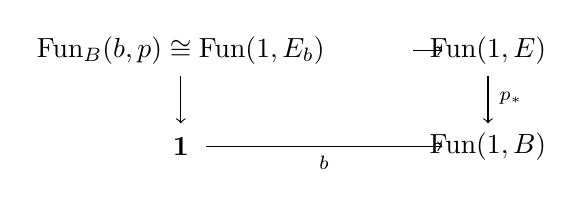
\begin{tikzpicture}[x=1.5em,y=1.5em]
  \node (fp) at (0,0) {$\mathrm{Fun}_{B}(b,p)\cong\mathrm{Fun}(1,E_{b})$};
  \node (fe) at (7.4,0) {$\mathrm{Fun}(1,E)$};
  \node (o)  at (0,-2.3) {$\qcOne$};
  \node (fb) at (7.4,-2.3) {$\mathrm{Fun}(1,B)$};
  \draw[->] (5.6,0) -- (6.3,0);
  \draw[->] (0,-0.6) -- (0,-1.75);
  \draw[->] (0.6,-2.3) -- node[below]{$\scriptstyle b$} (6.3,-2.3);
  \draw[->] (7.4,-0.6) -- (7.4,-1.75);
  \node at (7.95,-1.15) {$\scriptstyle p_{*}$};
  \node at (0.5,-0.52) {$\scriptstyle\llcorner$};
\end{tikzpicture}
\end{center}
它同构于 $p\colon E\twoheadrightarrow B$ 在 $b$ 之上的\trFiber{} $E_{b}$ 的%
\trUnderlyingQuasiCategory。
当 $p\colon E\twoheadrightarrow B$ 是离散等价纤维化时，$\mathrm{Fun}(1,E_{b})$
是一个\trKanComplex，且不妨更形象地称作\trFiber{} $E_{b}$ 的「底空间」。

如果把 $B$ 之上的一条\trDiscreteCartesianFibration{}想成一个是反变的、$B$-指标的、取值于离散
∞-范畴的函子，那么 $B$ 之上的\trDiscreteCartesianFibration{}之间的映射便是「\trNaturalTransformation」%
——之所以有
「在 $B$ 中的自然性」，是因为这些函子纤维化在 $B$ 之上。这就引出我们对纤维化式%
\trYonedaLemma{}的第一次陈述：

\begin{theorem}[离散 Yoneda 引理]\label{thm:discrete-yoneda-lemma}
若 $p\colon E\twoheadrightarrow B$ 是一条\trDiscreteCartesianFibration，则
\[
\mathrm{Fun}_{B}\bigl(\mathrm{Hom}_{B}(B,b)\xrightarrow{\ p_{0}\ }B,\,
E\xrightarrow{\ p\ }B\bigr)
\xrightarrow[\ \sim\ ]{\ \mathrm{ev}_{\qcor{\mathrm{id}_{b}}}\ }
\mathrm{Fun}(1,E_{b})
\]
是\trKanComplex{}之间的一个\trEquivalence。
\end{theorem}

我们从这样一个「依值」推广中推导出这一结果：其中作为靶的\trDiscreteCartesianFibration{}的余定义域
是 $\mathrm{Hom}_{B}(B,b)$。
在这一情形，该结果提供了\trDiscreteCartesianFibration
$q\colon F\twoheadrightarrow\mathrm{Hom}_{B}(B,b)$ 的诸\trSection{}与
$\qcor{\mathrm{id}_{b}}$ 之上\trFiber{}的诸\trElement{}之间的一个\trEquivalence。
这一结果类似于同伦类型论中恒等类型的「路径归纳」原理：
\cref{thm:dependent-yoneda-lemma}的逆等价提供了「搬运」运算的一个「有向」版本
[106, §9]。

\begin{theorem}[依值 Yoneda 引理]\label{thm:dependent-yoneda-lemma}
设 $b\colon\qcOne\to B$ 是一个∞-范畴 $B$ 中的一个元素，且
$q\colon F\twoheadrightarrow\mathrm{Hom}_{B}(B,b)$ 是一条\trDiscreteCartesianFibration，则
\[
\mathrm{Fun}_{\mathrm{Hom}_{B}(B,b)}\bigl(\mathrm{Hom}_{B}(B,b),F\bigr)
\xrightarrow[\ \sim\ ]{\ \mathrm{ev}_{\qcor{\mathrm{id}_{b}}}\ }
\mathrm{Fun}\bigl(1,F_{\qcor{\mathrm{id}_{b}}}\bigr)
\]
是\trKanComplex{}之间的一个\trEquivalence。
\end{theorem}

\cref{thm:discrete-yoneda-lemma}被一个允许 $p\colon E\twoheadrightarrow B$ 为任意%
\trCartesianFibration{}（不必离散）的推广所囊括。在这一情形，$p$ 编码一个反变的、
$B$-指标的、取值于∞-范畴的函子，正如 $p_{0}\colon\mathrm{Hom}_{B}(B,b)\twoheadrightarrow B$
所作的那样。两个这样的函子之间「\trNaturalTransformation」的正确概念现在由 $B$ 之上的笛卡尔函子给出
（见练习 5.3.iii）。
给定一对\trCartesianFibration{} $q\colon F\twoheadrightarrow B$ 与
$p\colon E\twoheadrightarrow B$，我们写作
\[
\mathrm{Fun}_{B}^{\mathrm{cart}}\bigl(F\xrightarrow{\ q\ }B,\,
E\xrightarrow{\ p\ }B\bigr)
\subset
\mathrm{Fun}_{B}\bigl(F\xrightarrow{\ q\ }B,\,
E\xrightarrow{\ p\ }B\bigr)
\]
表示由其顶点定义从 $q$ 到 $p$ 的笛卡尔函子的那些单纯形全体组成的子拟范畴。
\footnote{对任何拟范畴 $Q$ 与其顶点的任何子集，都存在一个「满」子拟范畴，它恰好
包含这些顶点以及 $Q$ 中由它们张出的全部单纯形。}

\begin{theorem}[\trYonedaLemma]\label{thm:yoneda-lemma}
若 $p\colon E\twoheadrightarrow B$ 是一条\trCartesianFibration，则
\[
\mathrm{Fun}_{B}^{\mathrm{cart}}\bigl(\mathrm{Hom}_{B}(B,b)
\xrightarrow{\ p_{0}\ }B,\,
E\xrightarrow{\ p\ }B\bigr)
\xrightarrow[\ \sim\ ]{\ \mathrm{ev}_{\qcor{\mathrm{id}_{b}}}\ }
\mathrm{Fun}(1,E_{b})
\]
是拟范畴之间的一个\trEquivalence。
\end{theorem}

这些定理的证明大范围地相互交叠，我们将平行地展开它们。基本想法是利用
$\qcor{\mathrm{id}_{b}}$ 作为 $\mathrm{Hom}_{B}(B,b)$ 在∞-宇宙 $\mathcal{K}$ 中的
一个\trTerminal{}元素的\trUniversalProperty（见推论 3.5.10）来为
$\mathrm{ev}_{\qcor{\mathrm{id}_{b}}}$ 定义一个\trRightAdjoint，并证明：当
$p\colon E\twoheadrightarrow B$ 是离散的、或当定义域被限制到笛卡尔函子的子拟范畴时，
这一伴随定义了一个\trAdjointEquivalence。
注意，函子 $\mathrm{ev}_{\qcor{\mathrm{id}_{b}}}$ 是函子 $\qcor{\mathrm{id}_{b}}$
在 2-函子 $\mathrm{Fun}_{B}(-,p)\colon\hbar(\mathcal{K}_{/B})^{\mathrm{op}}\to\hQCat$
之下的像。若伴随 $!\dashv\qcor{\mathrm{id}_{b}}$ 生活在切片∞-宇宙
$\mathcal{K}_{/B}$ 之中，这就会直接构造出 $\mathrm{ev}_{\qcor{\mathrm{id}_{b}}}$
的一个\trRightAdjoint。贯彻这一思路的主要技术困难在于：见证
$\qcor{\mathrm{id}_{b}}$ 之终性的那个伴随并不生活在同伦 2-范畴的切片
$\hK_{/B}$ 中，而是生活在同伦 2-范畴的一个我们现在即将引入的松弛切片
$\hK_{/\!\!/B}$ 中。

\begin{definition}[松弛切片 2-范畴]\label{def:lax-slice}
考虑一个 2-范畴 $\hK$ 与一个对象 $A\in\hK$。%
\textbf{松弛切片 2-范畴}（lax slice 2-category）$\hK_{/\!\!/A}$ 是这样一个严格
2-范畴，其
\begin{itemize}
\item 对象是 $\hK$ 中余定义域为 $A$ 的映射 $f\colon X\to A$；
\item 1-胞腔是 $\hK$ 中的图表
\begin{rveq}\label{eq:lax-slice-cell}
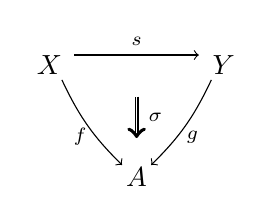
\begin{tikzpicture}[x=1.5em,y=1.5em]
  \node (X) at (0,1.2) {$X$};
  \node (Y) at (4.2,1.2) {$Y$};
  \node (A) at (2.1,-1.5) {$A$};
  \draw[->] (0.6,1.45) -- node[above]{$\scriptstyle s$} (3.6,1.45);
  \draw[->] (0.3,0.85) to[bend right=10] node[left,pos=0.65]{$\scriptstyle f$} (1.75,-1.2);
  \draw[->] (3.9,0.85) to[bend left=10] node[right,pos=0.65]{$\scriptstyle g$} (2.45,-1.2);
  \draw[double,->] (2.1,0.45) -- (2.1,-0.55);
  \node at (2.55,-0.05) {$\scriptstyle\sigma$};
\end{tikzpicture}
\end{rveq}
以及
\item 从 $(s,\sigma)$ 到 $(s',\sigma')$ 的 2-胞腔是使得下式成立的 2-胞腔
$\theta\colon s\Rightarrow s'$：
\begin{rveq}\label{eq:lax-slice-2cell}
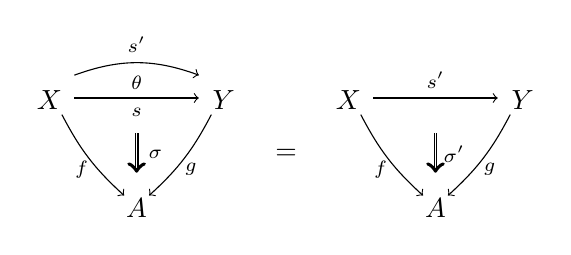
\begin{tikzpicture}[x=1.5em,y=1.5em]
  \begin{scope}[shift={(0,0)}]
  \node (X) at (0,0.9) {$X$};
  \node (Y) at (4.2,0.9) {$Y$};
  \node (A) at (2.1,-1.7) {$A$};
  \draw[->] (0.6,1.5) to[bend left=20] node[above]{$\scriptstyle s'$} (3.6,1.5);
  \draw[->] (0.6,0.95) -- node[below]{$\scriptstyle s$} (3.6,0.95);
  \node at (2.1,1.32) {$\scriptstyle\theta$};
  \draw[->] (0.3,0.55) to[bend right=10] node[left,pos=0.65]{$\scriptstyle f$} (1.8,-1.4);
  \draw[->] (3.9,0.55) to[bend left=10] node[right,pos=0.65]{$\scriptstyle g$} (2.4,-1.4);
  \draw[double,->] (2.1,0.1) -- (2.1,-0.85);
  \node at (2.55,-0.4) {$\scriptstyle\sigma$};
  \end{scope}
  \node at (5.7,-0.4) {$=$};
  \begin{scope}[shift={(7.2,0)}]
  \node (X) at (0,0.9) {$X$};
  \node (Y) at (4.2,0.9) {$Y$};
  \node (A) at (2.1,-1.7) {$A$};
  \draw[->] (0.6,0.95) -- node[above]{$\scriptstyle s'$} (3.6,0.95);
  \draw[->] (0.3,0.55) to[bend right=10] node[left,pos=0.65]{$\scriptstyle f$} (1.8,-1.4);
  \draw[->] (3.9,0.55) to[bend left=10] node[right,pos=0.65]{$\scriptstyle g$} (2.4,-1.4);
  \draw[double,->] (2.1,0.1) -- (2.1,-0.85);
  \node at (2.55,-0.4) {$\scriptstyle\sigma'$};
  \end{scope}
\end{tikzpicture}
\end{rveq}
\end{itemize}
\end{definition}

例如，定义\trTerminal{}元素的诸伴随可提升到松弛切片 2-范畴中：

\begin{lemma}\label{lem:terminal-lax-slice-adjunction}
设 $t\colon\qcOne\to A$ 在∞-宇宙 $\mathcal{K}$ 中的一个∞-范畴 $A$ 里定义了一个%
\trTerminal{}元素。那么
\begin{center}
\begin{tikzpicture}[x=1.5em,y=1.5em]
  \begin{scope}[shift={(0,0)}]
  \node (o) at (0,1.2) {$\qcOne$};
  \node (A1) at (3.6,1.2) {$A$};
  \node (A2) at (1.8,-1.3) {$A$};
  \draw[->] (0.55,1.45) -- node[above]{$\scriptstyle t$} (3.05,1.45);
  \draw[->] (0.3,0.85) to[bend right=12] node[left,pos=0.6]{$\scriptstyle t$} (1.5,-1.05);
  \draw[double] (2.3,-0.6) -- (3.5,0.9);
  \end{scope}
  \node[align=center] at (6.7,0.1) {右伴随于\\单位映射};
  \begin{scope}[shift={(9.2,0)}]
  \node (A1) at (0,1.2) {$A$};
  \node (o)  at (3.6,1.2) {$\qcOne$};
  \node (A2) at (1.8,-1.3) {$A$};
  \draw[->] (0.55,1.45) -- node[above]{$\scriptstyle !$} (3.05,1.45);
  \draw[double] (0,0.85) -- (0,-0.7);
  \node at (-0.75,0.1) {$\scriptstyle\eta$};
  \draw[->] (3.35,0.85) to[bend left=12] node[right,pos=0.6]{$\scriptstyle t$} (2.15,-1.05);
  \end{scope}
\end{tikzpicture}
\end{center}
于松弛切片 2-范畴 $\hK_{/\!\!/A}$ 中。
\end{lemma}

\begin{proof}
我们来验证：见证 $t$ 之终性的伴随 $!\dashv t$ 的\trUnit{}与\trCounit{}沿遗忘
2-函子 $\hK_{/\!\!/A}\to\hK$ 提升；这归结为验证条件
\eqref{eq:lax-slice-2cell}。遗忘 2-函子 $\hK_{/\!\!/A}\to\hK$ 在 1-与 2-胞腔上是%
\trFaithful，故诸三角等式对被提升的胞腔自动成立。这些松弛相容性条件归结为下列
粘贴等式
\begin{center}
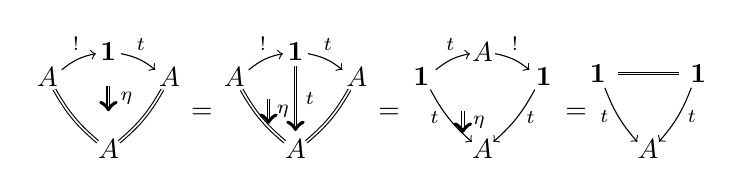
\begin{tikzpicture}[x=1.3em,y=1.3em]
  \begin{scope}[shift={(0,0)}]
  \node (a1) at (-1.7,0.8) {$A$};
  \node (o1) at (0,1.5) {$\qcOne$};
  \node (a2) at (1.7,0.8) {$A$};
  \node (a3) at (0,-1.2) {$A$};
  \draw[->] (-1.3,1.0) to[bend left=14] node[above,pos=0.45]{$\scriptstyle !$} (-0.35,1.45);
  \draw[->] (0.35,1.45) to[bend left=14] node[above,pos=0.55]{$\scriptstyle t$} (1.3,1.0);
  \draw[double] (-1.5,0.45) to[bend right=10] (-0.3,-1.0);
  \draw[double] (1.5,0.45) to[bend left=10] (0.3,-1.0);
  \draw[double,->] (0,0.55) -- (0,-0.15);
  \node at (0.5,0.2) {$\scriptstyle\eta$};
  \end{scope}
  \node at (2.6,-0.2) {$=$};
  \begin{scope}[shift={(5.2,0)}]
  \node (a1) at (-1.7,0.8) {$A$};
  \node (o1) at (0,1.5) {$\qcOne$};
  \node (a2) at (1.7,0.8) {$A$};
  \node (a3) at (0,-1.2) {$A$};
  \draw[->] (-1.3,1.0) to[bend left=14] node[above,pos=0.45]{$\scriptstyle !$} (-0.35,1.45);
  \draw[->] (0.35,1.45) to[bend left=14] node[above,pos=0.55]{$\scriptstyle t$} (1.3,1.0);
  \draw[double] (-1.5,0.45) to[bend right=10] (-0.3,-1.0);
  \draw[double,->] (0,1.1) -- (0,-0.7);
  \node at (0.4,0.2) {$\scriptstyle t$};
  \draw[double] (1.5,0.45) to[bend left=10] (0.3,-1.0);
  \draw[double,->] (-0.75,0.2) -- (-0.75,-0.5);
  \node at (-0.35,-0.15) {$\scriptstyle\eta$};
  \end{scope}
  \node at (7.8,-0.2) {$=$};
  \begin{scope}[shift={(10.4,0)}]
  \node (o1) at (-1.7,0.8) {$\qcOne$};
  \node (a1) at (0,1.5) {$A$};
  \node (o2) at (1.7,0.8) {$\qcOne$};
  \node (a3) at (0,-1.2) {$A$};
  \draw[->] (-1.3,1.0) to[bend left=14] node[above,pos=0.45]{$\scriptstyle t$} (-0.35,1.45);
  \draw[->] (0.35,1.45) to[bend left=14] node[above,pos=0.55]{$\scriptstyle !$} (1.3,1.0);
  \draw[->] (-1.45,0.45) to[bend right=10] node[left,pos=0.5]{$\scriptstyle t$} (-0.3,-1.0);
  \draw[->] (1.45,0.45) to[bend left=10] node[right,pos=0.5]{$\scriptstyle t$} (0.3,-1.0);
  \draw[double,->] (-0.55,-0.15) -- (-0.55,-0.75);
  \node at (-0.1,-0.45) {$\scriptstyle\eta$};
  \end{scope}
  \node at (13.0,-0.2) {$=$};
  \begin{scope}[shift={(15.0,0)}]
  \node (o1) at (-1.4,0.9) {$\qcOne$};
  \node (o2) at (1.4,0.9) {$\qcOne$};
  \node (a3) at (0,-1.2) {$A$};
  \draw[double] (-0.85,0.9) -- (0.85,0.9);
  \draw[->] (-1.2,0.5) to[bend right=10] node[left,pos=0.5]{$\scriptstyle t$} (-0.3,-1.0);
  \draw[->] (1.2,0.5) to[bend left=10] node[right,pos=0.5]{$\scriptstyle t$} (0.3,-1.0);
  \end{scope}
\end{tikzpicture}
\end{center}
其中第一式是平凡的，而第二式由\trTriangleEqualities{}
$\eta t=\mathrm{id}_{t}$ 成立。
\end{proof}

利用多少有些非标准的 2-范畴技巧，我们把\cref{lem:terminal-lax-slice-adjunction}
的伴随转移为一个\trAdjointEquivalence
\begin{center}
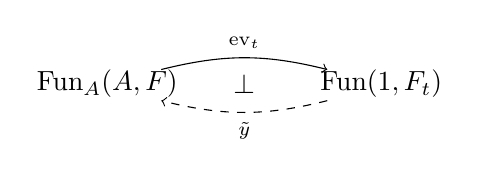
\begin{tikzpicture}[x=1.5em,y=1.5em]
  \node (L) at (0,0) {$\mathrm{Fun}_{A}(A,F)$};
  \node (R) at (6.6,0) {$\mathrm{Fun}(1,F_{t})$};
  \draw[->] (1.3,0.35) to[bend left=14] node[above]{$\scriptstyle\mathrm{ev}_{t}$} (5.3,0.35);
  \node at (3.3,0) {$\perp$};
  \draw[->,dashed] (5.3,-0.4) to[bend left=14] node[below]{$\scriptstyle\tilde{y}$} (1.3,-0.4);
\end{tikzpicture}
\end{center}
它连接一条\trDiscreteCartesianFibration{} $q\colon F\twoheadrightarrow A$ 的诸\trSection{}之%
\trKanComplex{}与\trFiber{} $F_{t}$ 在一个\trTerminal{}元素 $t\colon\qcOne\to A$ 之上的
底空间。由于我们最初的伴随生活在松弛切片而非严格切片之中，这一构造颇为精微，
要经过一对我们即将引入的辅助 2-范畴。

\begin{definition}\label{def:cospan-2category}
设 $\hK$ 是某个∞-宇宙的同伦 2-范畴，并以 $\hK^{\perp}$ 记这样一个严格
2-范畴，其
\begin{itemize}
\item 对象是余跨度
\[
A\xrightarrow{\ k\ }B\xleftarrow{\ p\ }E
\]
其中 $p$ 是一条\trCartesianFibration；
\item 1-胞腔是形如下式的图表
\begin{rveq}\label{eq:cospan-1cell}
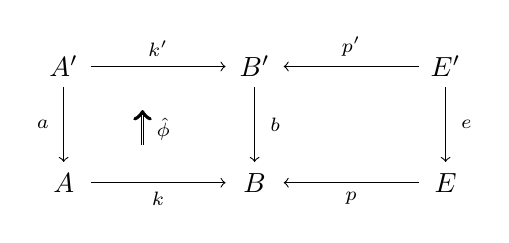
\begin{tikzpicture}[x=1.5em,y=1.5em]
  \node (Ap) at (0,1.4) {$A'$};
  \node (Bp) at (4.6,1.4) {$B'$};
  \node (Ep) at (9.2,1.4) {$E'$};
  \node (A)  at (0,-1.4) {$A$};
  \node (B)  at (4.6,-1.4) {$B$};
  \node (E)  at (9.2,-1.4) {$E$};
  \draw[->] (0.65,1.4) -- node[above]{$\scriptstyle k'$} (3.9,1.4);
  \draw[->] (8.55,1.4) -- node[above]{$\scriptstyle p'$} (5.3,1.4);
  \draw[->] (0.65,-1.4) -- node[below]{$\scriptstyle k$} (3.9,-1.4);
  \draw[->] (8.55,-1.4) -- node[below]{$\scriptstyle p$} (5.3,-1.4);
  \draw[->] (0,0.9) -- (0,-0.9);  \node at (-0.5,0) {$\scriptstyle a$};
  \draw[->] (4.6,0.9) -- (4.6,-0.9);  \node at (5.1,0) {$\scriptstyle b$};
  \draw[->] (9.2,0.9) -- (9.2,-0.9);  \node at (9.7,0) {$\scriptstyle e$};
  \draw[double,->] (1.9,-0.5) -- (1.9,0.35);
  \node at (2.4,-0.1) {$\scriptstyle\hat{\phi}$};
\end{tikzpicture}
\end{rveq}
以及
\item 其 2-胞腔由平行 1-胞腔图表之诸竖直边之间的三元组
$\alpha\colon a\Rightarrow\bar{a}$、$\beta\colon b\Rightarrow\bar{b}$ 与
$\epsilon\colon e\Rightarrow\bar{e}$ 构成，满足 $p\epsilon=\beta p'$ 与
$\bar{\phi}\cdot k\alpha=\beta k'\cdot\hat{\phi}$。
\end{itemize}
\end{definition}

\begin{definition}\label{def:pullback-square-2category}
设 $\hK$ 是某个∞-宇宙的同伦 2-范畴，并以 $\hK^{\square}$ 记这样一个严格
2-范畴，其
\begin{itemize}
\item 对象是诸拉回方块
\begin{center}
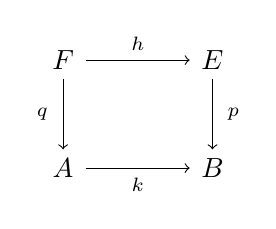
\begin{tikzpicture}[x=1.5em,y=1.5em]
  \node (F) at (0,1.3) {$F$};
  \node (E) at (3.6,1.3) {$E$};
  \node (A) at (0,-1.3) {$A$};
  \node (B) at (3.6,-1.3) {$B$};
  \draw[->] (0.55,1.3) -- node[above]{$\scriptstyle h$} (3.05,1.3);
  \draw[->] (0,0.85) -- (0,-0.85);  \node at (-0.5,0) {$\scriptstyle q$};
  \draw[->] (3.6,0.85) -- (3.6,-0.85);  \node at (4.1,0) {$\scriptstyle p$};
  \draw[->] (0.55,-1.3) -- node[below]{$\scriptstyle k$} (3.05,-1.3);
  \node at (0.5,0.82) {$\scriptstyle\llcorner$};
\end{tikzpicture}
\end{center}
其诸竖直边均为\trCartesianFibration；
\item 1-胞腔是诸立方体
\begin{rveq}\label{eq:pullback-cube}
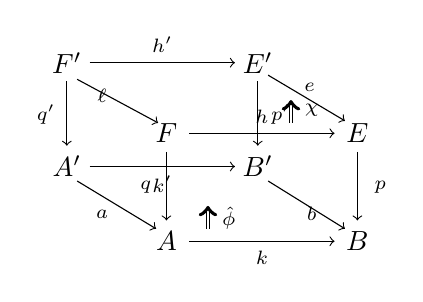
\begin{tikzpicture}[x=1.5em,y=1.5em]
  \node (Fp) at (0,3.4) {$F'$};
  \node (Ep) at (4.6,3.4) {$E'$};
  \node (Ap) at (0,0.9) {$A'$};
  \node (Bp) at (4.6,0.9) {$B'$};
  \draw[->] (0.55,3.4) -- node[above]{$\scriptstyle h'$} (4.05,3.4);
  \draw[->] (0,2.95) -- (0,1.4);  \node at (-0.5,2.15) {$\scriptstyle q'$};
  \draw[->] (4.6,2.95) -- (4.6,1.4);  \node at (5.15,2.15) {$\scriptstyle p'$};
  \draw[->] (0.55,0.9) -- node[below]{$\scriptstyle k'$} (4.05,0.9);
  \node (F) at (2.4,1.7) {$F$};
  \node (E) at (7.0,1.7) {$E$};
  \node (A) at (2.4,-0.9) {$A$};
  \node (B) at (7.0,-0.9) {$B$};
  \draw[->] (2.95,1.7) -- node[above]{$\scriptstyle h$} (6.45,1.7);
  \draw[->] (2.4,1.25) -- (2.4,-0.4);  \node at (1.9,0.4) {$\scriptstyle q$};
  \draw[->] (7.0,1.25) -- (7.0,-0.4);  \node at (7.55,0.4) {$\scriptstyle p$};
  \draw[->] (2.95,-0.9) -- node[below]{$\scriptstyle k$} (6.45,-0.9);
  \draw[->] (0.25,3.0) -- (2.2,1.95);  \node at (0.85,2.6) {$\scriptstyle\ell$};
  \draw[->] (4.85,3.1) -- (6.7,2.0);  \node at (5.85,2.8) {$\scriptstyle e$};
  \draw[->] (0.25,0.55) -- (2.15,-0.6);  \node at (0.85,-0.25) {$\scriptstyle a$};
  \draw[->] (4.85,0.55) -- (6.7,-0.6);  \node at (5.9,-0.25) {$\scriptstyle b$};
  \draw[double,->] (5.4,1.95) -- (5.4,2.5);
  \node at (5.9,2.25) {$\scriptstyle\chi$};
  \draw[double,->] (3.4,-0.6) -- (3.4,-0.05);
  \node at (3.9,-0.35) {$\scriptstyle\hat{\phi}$};
\end{tikzpicture}
\end{rveq}
其诸竖直面交换，且其中 $\chi\colon h\ell\Rightarrow eh'$ 是 $\hat{\phi}q'$ 的一个
$p$-笛卡尔提升；以及
\item 其 2-胞腔由四元组 $\alpha\colon a\Rightarrow\bar{a}$、
$\beta\colon b\Rightarrow\bar{b}$、$\epsilon\colon e\Rightarrow\bar{e}$ 与
$\lambda\colon\ell\Rightarrow\bar{\ell}$ 给出，其中 $\epsilon$ 与 $\lambda$
分别是 $\beta p'$ 与 $\alpha q'$ 的提升，且满足
$\bar{\phi}\cdot k\alpha=\beta k'\cdot\hat{\phi}$ 与
$\bar{\chi}\cdot h\lambda=\epsilon h'\cdot\chi$。
\end{itemize}
\end{definition}

这些定义的安排方式使得有一个显然的遗忘 2-函子
$U\colon\hK^{\square}\to\hK^{\perp}$，它具有定义 3.6.1 中引入的强满射性质。

\begin{lemma}\label{lem:smothering-forgetful}
遗忘 2-函子 $U\colon\hK^{\square}\to\hK^{\perp}$ 是一个覆盖 2-函子。
\end{lemma}

\begin{proof}
命题 5.2.4 告诉我们 $\hK^{\square}\to\hK^{\perp}$ 在对象上是满的。
为证它在 1-胞腔上是满的，先对 \eqref{eq:cospan-1cell} 中的诸余跨度作\trPullback，
然后将 $\chi$ 定义为 $\hat{\phi}q'$ 的、以 $eh'$ 为余定义域的任意一支 $p$-笛卡尔
提升。由构造，$\chi$ 的定义域严格地位于 $kaq'$ 之上，于是这个函子唯一地穿过定义
\eqref{eq:pullback-cube} 中映射 $\ell$ 的那条\trPullback{}腿 $h$ 而分解。

为证 $\hK^{\square}\to\hK^{\perp}$ 在 2-胞腔上是满的，考虑 $\hK^{\square}$ 中
一对平行的 1-胞腔。对其一我们使用 \eqref{eq:pullback-cube} 的记号，对另一支我们
把诸对角函子记作 $\bar{a}$、$\bar{b}$、$\bar{e}$ 与 $\bar{\ell}$，并把诸 2-胞腔
记作 $\bar{\phi}$ 与 $\bar{\chi}$；这些 1-胞腔须平行的要求蕴含诸\trPullback{}面
必然相同。现在考虑满足\cref{def:cospan-2category}诸条件的三元组
$\alpha\colon a\Rightarrow\bar{a}$、$\beta\colon b\Rightarrow\bar{b}$ 与
$\epsilon\colon e\Rightarrow\bar{e}$。我们的任务是定义第四个 2-胞腔
$\lambda\colon\ell\Rightarrow\bar{\ell}$，使得 $q\lambda=\alpha q'$ 且
$\bar{\chi}\cdot h\lambda=\epsilon h'\cdot\chi$。

为达到这一目的，我们先用 $p$-笛卡尔胞腔
$\bar{\chi}\colon h\bar{\ell}\Rightarrow\bar{e}h'$ 的归纳性质，对复合 2-胞腔
$\epsilon h'\cdot\chi\colon h\ell\Rightarrow\bar{e}h'$ 与分解
$p\epsilon h'\cdot p\chi=\bar{\phi}q'\cdot k\alpha q'$ 定义一个 2-胞腔
$\gamma\colon h\ell\Rightarrow h\bar{\ell}$。
由构造 $p\gamma=k\alpha q'$，于是偶对 $\alpha q'$ 与 $\gamma$ 诱导出一个 2-胞腔
$\lambda\colon\ell\Rightarrow\bar{\ell}$，使得 $q\lambda=\alpha q'$ 且
$h\lambda=\gamma$。四元组 $(\alpha,\beta,\epsilon,\lambda)$ 现在定义了
$\hK^{\square}$ 中所需的 2-胞腔。

最后，对于 2-胞腔保守性：设 $\alpha$、$\beta$ 与 $\epsilon$ 如上均为同构。由
命题 3.3.1 所述\trPullback{}的保守性性质，为证 $\lambda$ 是一个\trIsomorphism，
只需证 $q\lambda=\alpha q'$ 是（这我们已知）且 $h\lambda=\gamma$ 可逆。
但 $\gamma$ 是作为分解 $\epsilon h'\cdot\chi=\bar{\chi}\cdot\gamma$（满足
$p\gamma=k\alpha q'$）构造出来的。由于 $\epsilon$ 是一个\trIsomorphism，
$\epsilon h'\cdot\chi$ 是 $p$-笛卡尔的，故引理 5.1.12 证明 $\gamma$ 是一个%
\trIsomorphism。
\end{proof}

我们无法在同伦 2-范畴中直接定义一个拉回 2-函子 $\hK^{\perp}\to\hK$，因为 $\hK$
中诸\trPullback{}的 2-范畴式\trUniversalProperty{}是弱的而非严格的（见命题
3.3.1）。
作为替代，2-函子之锯齿
\begin{center}
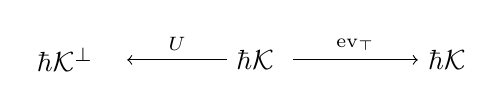
\begin{tikzpicture}[x=1.5em,y=1.5em]
  \node (kp) at (0,0) {$\hK^{\perp}$};
  \node (ks) at (4.6,0) {$\hK^{\square}$};
  \node (k)  at (9.2,0) {$\hK$};
  \draw[->] (3.9,0) -- node[above]{$\scriptstyle U$} (1.5,0);
  \draw[->] (5.5,0) -- node[above]{$\scriptstyle\mathrm{ev}_{\top}$} (8.5,0);
\end{tikzpicture}
\end{center}
——其中逆向映射是一个覆盖 2-函子，而前向映射在\trPullback{}顶点处求值——定义了
一个合理的替身。

\begin{proposition}\label{prop:evaluation-right-adjoint}
设 $t\colon\qcOne\to A$ 定义了 $A$ 的一个\trTerminal{}元素，并设
$q\colon F\twoheadrightarrow A$ 是一条\trCartesianFibration。那么在 $t$
处的求值容有一个\trRightAdjoint
\begin{center}
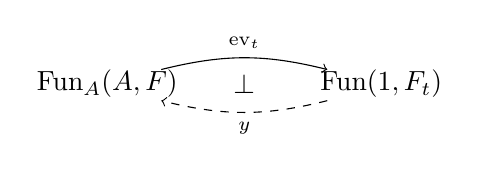
\begin{tikzpicture}[x=1.5em,y=1.5em]
  \node (L) at (0,0) {$\mathrm{Fun}_{A}(A,F)$};
  \node (R) at (6.6,0) {$\mathrm{Fun}(1,F_{t})$};
  \draw[->] (1.3,0.35) to[bend left=14] node[above]{$\scriptstyle\mathrm{ev}_{t}$} (5.3,0.35);
  \node at (3.3,0) {$\perp$};
  \draw[->,dashed] (5.3,-0.4) to[bend left=14] node[below]{$\scriptstyle y$} (1.3,-0.4);
\end{tikzpicture}
\end{center}
使得当 $q$ 是一条\trDiscreteCartesianFibration{}时，它定义\trKanComplex{}之间的一个%
\trAdjointEquivalence。
\end{proposition}

\begin{proof}
所求的\trAdjunction{}是这样得到的：把\cref{lem:terminal-lax-slice-adjunction}
的伴随穿过如下的 2-函子序列而转移
\begin{center}
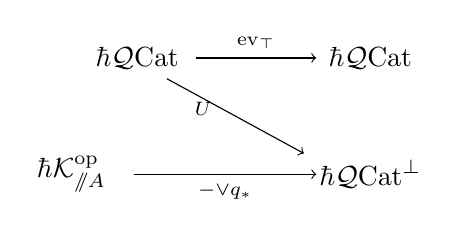
\begin{tikzpicture}[x=1.5em,y=1.5em]
  \node (qs) at (1.0,1.4) {$\hQCat^{\square}$};
  \node (q)  at (6.6,1.4) {$\hQCat$};
  \node (kl) at (-0.6,-1.4) {$\hK_{/\!\!/A}^{\mathrm{op}}$};
  \node (qp) at (6.6,-1.4) {$\hQCat^{\perp}$};
  \draw[->] (2.4,1.4) -- node[above]{$\scriptstyle\mathrm{ev}_{\top}$} (5.3,1.4);
  \draw[->] (1.7,0.9) -- node[left,pos=0.4]{$\scriptstyle U$} (5.0,-0.9);
  \draw[->] (0.9,-1.4) -- node[below]{$\scriptstyle-\vee q_{*}$} (5.3,-1.4);
\end{tikzpicture}
\end{center}
并利用引理 3.6.7 沿中间的覆盖 2-函子提升。

对∞-宇宙 $\mathcal{K}$ 中一条固定的\trCartesianFibration{}
$q\colon F\twoheadrightarrow A$，有一个 2-函子
$-\vee q_{*}\colon\hK_{/\!\!/A}^{\mathrm{op}}\to\hQCat^{\perp}$，它把一个 1-胞腔
\eqref{eq:lax-slice-cell} 送到
\begin{center}
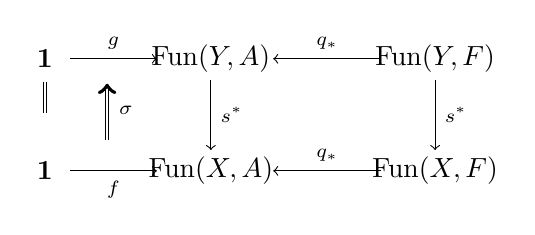
\begin{tikzpicture}[x=1.5em,y=1.5em]
  \node (o1) at (0,1.2) {$\qcOne$};
  \node (ga) at (4.0,1.2) {$\mathrm{Fun}(Y,A)$};
  \node (gf) at (9.4,1.2) {$\mathrm{Fun}(Y,F)$};
  \node (o2) at (0,-1.5) {$\qcOne$};
  \node (fa) at (4.0,-1.5) {$\mathrm{Fun}(X,A)$};
  \node (ff) at (9.4,-1.5) {$\mathrm{Fun}(X,F)$};
  \draw[->] (0.6,1.2) -- node[above]{$\scriptstyle g$} (2.7,1.2);
  \draw[->] (8.1,1.2) -- node[above]{$\scriptstyle q_{*}$} (5.5,1.2);
  \draw[->] (8.1,-1.5) -- node[above]{$\scriptstyle q_{*}$} (5.5,-1.5);
  \draw[double] (0,-0.1) -- (0,0.65);
  \draw[double,->] (1.5,-0.75) -- (1.5,0.6);
  \node at (1.95,-0.05) {$\scriptstyle\sigma$};
  \draw[->] (4.0,0.7) -- (4.0,-1.0);  \node at (4.5,-0.15) {$\scriptstyle s^{*}$};
  \draw[->] (9.4,0.7) -- (9.4,-1.0);  \node at (9.9,-0.15) {$\scriptstyle s^{*}$};
  \draw[->] (0.6,-1.5) -- node[below]{$\scriptstyle f$} (2.7,-1.5);
\end{tikzpicture}
\end{center}
并把一个 2-胞腔 $\theta\colon s\Rightarrow s'$ 送到那个在其两个非恒同分量处经与
$\theta$ 作前须化而作用的 2-胞腔。
由推论 5.3.5，诸函子 $q_{*}$ 是拟范畴的\trCartesianFibration。

现在，我们把 2-函子 $-\vee q_{*}\colon\hK_{/\!\!/A}^{\mathrm{op}}\to\hQCat^{\perp}$
应用于\cref{lem:terminal-lax-slice-adjunction}的伴随以得到 $\hQCat^{\perp}$ 中的
一个\trAdjunction，然后用\cref{lem:smothering-forgetful}的覆盖 2-函子与引理
3.6.7 把它提升为 $\hQCat^{\square}$ 中的一个\trAdjunction。
如练习 3.6.iii 所详述，$\hQCat^{\square}$ 中被提升的\trAdjunction{}可以用
$\hQCat^{\perp}$ 中\trAdjunction{}之对象、1-胞腔以及单位或余单位（任取其一）的
任意提升构造出来。

特别地，我们可以取 $\hQCat^{\square}$ 中被提升\trAdjunction{}的左、右伴随为
$\hK_{/\!\!/A}$ 中\trAdjunction{} $!\dashv t$ 之右、左伴随在 $\hQCat^{\perp}$
中之像的任意提升：
\begin{rveq}\label{eq:yoneda-transfer-cube}
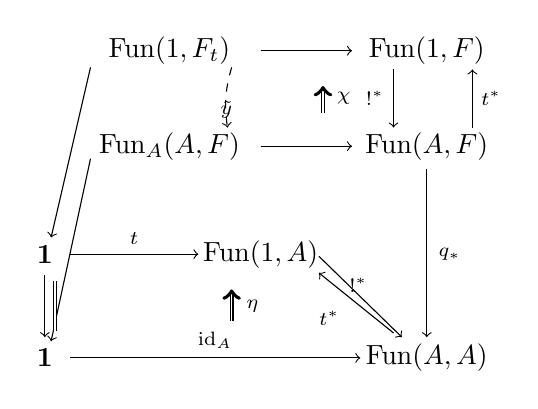
\begin{tikzpicture}[x=1.5em,y=1.5em]
  \node (Ft) at (0,3.4) {$\mathrm{Fun}(1,F_{t})$};
  \node (F1) at (6.2,3.4) {$\mathrm{Fun}(1,F)$};
  \node (FA) at (0,1.1) {$\mathrm{Fun}_{A}(A,F)$};
  \node (F)  at (6.2,1.1) {$\mathrm{Fun}(A,F)$};
  \node (o1) at (-3.0,-1.5) {$\qcOne$};
  \node (F1A) at (2.2,-1.5) {$\mathrm{Fun}(1,A)$};
  \node (o2) at (-3.0,-4.0) {$\qcOne$};
  \node (AA) at (6.2,-4.0) {$\mathrm{Fun}(A,A)$};
  \draw[->] (2.2,3.4) -- (4.4,3.4);
  \draw[->] (2.2,1.1) -- (4.4,1.1);
  \draw[->,dashed] (1.5,3.0) to[bend right=12] node[below,pos=0.4]{$\scriptstyle\tilde{y}$} (1.4,1.55);
  \draw[->] (5.4,2.95) -- (5.4,1.55);  \node at (4.95,2.25) {$\scriptstyle!^{*}$};
  \draw[->] (7.3,1.55) -- (7.3,2.95);  \node at (7.75,2.25) {$\scriptstyle t^{*}$};
  \draw[double,->] (3.7,1.9) -- (3.7,2.55);  %
  \node at (4.2,2.25) {$\scriptstyle\chi$};
  \draw[->] (-1.9,3.0) -- (-2.85,-1.1);
  \draw[->] (-1.9,0.8) -- (-2.85,-3.6);
  \node at (1.1,2.9) {$\scriptstyle\llcorner$};
  \node at (1.0,0.6) {$\scriptstyle\llcorner$};
  \draw[->] (6.2,0.55) -- (6.2,-3.5);  \node at (6.75,-1.5) {$\scriptstyle q_{*}$};
  \draw[->] (-3.0,-2.0) -- (-3.0,-3.5);
  \draw[double] (-2.75,-2.15) -- (-2.75,-3.35);
  \draw[->] (-2.4,-1.5) -- node[above]{$\scriptstyle t$} (0.7,-1.5);
  \draw[->] (3.6,-1.55) -- (5.6,-3.5);  \node at (4.55,-2.25) {$\scriptstyle!^{*}$};
  \draw[->] (5.4,-3.4) -- (3.6,-1.95);  \node at (3.85,-3.05) {$\scriptstyle t^{*}$};
  \draw[double,->] (1.5,-3.1) -- (1.5,-2.35);
  \node at (2.0,-2.75) {$\scriptstyle\eta$};
  \draw[->] (-2.4,-4.0) -- node[above]{$\scriptstyle\mathrm{id}_{A}$} (4.6,-4.0);
\end{tikzpicture}
\end{rveq}
这表明左伴随就是所求的函子。由于 $!\dashv t$ 的\trCounit{}是一个恒同，被提升%
\trAdjunction{}的\trCounit{}也可取为恒同。最后，我们与在\trPullback{}顶点处求值
的遗忘 2-函子 $\hQCat^{\square}\to\hQCat$ 复合，把我们在 $\hQCat^{\square}$ 中的%
\trAdjunction{}投射为 $\hQCat$ 中所求的\trAdjunction。

当 $q\colon F\twoheadrightarrow A$ 是离散等价纤维化时，$\mathrm{Fun}(1,F_{t})$
与 $\mathrm{Fun}_{A}(A,F)$ 都是\trKanComplex{}。\trKanComplex{}之间的任何%
\trAdjunction{}自动是一个\trAdjointEquivalence，因为由推论 1.1.22 可知：余定义
域为\trKanComplex{}的任何\trNaturalTransformation{}都是自然同构。
\end{proof}

\cref{prop:evaluation-right-adjoint}的一个特例证明了依值 Yoneda 引理。

\begin{proof}[\cref{thm:dependent-yoneda-lemma}的证明]
回忆推论 3.5.10：对任意元素 $b\colon\qcOne\to B$，其恒同箭头
$\qcor{\mathrm{id}_{b}}\colon\qcOne\to\mathrm{Hom}_{B}(B,b)$ 定义了一个%
\trTerminal{}元素。
于是，依值 Yoneda 引理作为\cref{prop:evaluation-right-adjoint}的特例立即可得。
\end{proof}

利用\cref{thm:dependent-yoneda-lemma}，我们现在证明离散 Yoneda 引理。

\begin{proof}[\cref{thm:discrete-yoneda-lemma}的证明]
设 $p\colon E\twoheadrightarrow B$ 是一条\trDiscreteCartesianFibration，并考虑一个元素
$b\colon\qcOne\to B$。由引理 5.5.5，\trPullback
\begin{rveq}\label{eq:representable-pullback}
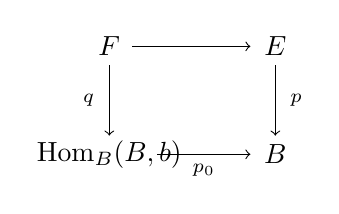
\begin{tikzpicture}[x=1.5em,y=1.5em]
  \node (F) at (0,1.3) {$F$};
  \node (E) at (4.0,1.3) {$E$};
  \node (H) at (0,-1.3) {$\mathrm{Hom}_{B}(B,b)$};
  \node (B) at (4.0,-1.3) {$B$};
  \draw[->] (0.55,1.3) -- (3.4,1.3);
  \draw[->] (0,0.85) -- (0,-0.85);  \node at (-0.5,0) {$\scriptstyle q$};
  \draw[->] (4.0,0.85) -- (4.0,-0.85);  \node at (4.5,0) {$\scriptstyle p$};
  \draw[->] (1.15,-1.3) -- node[below]{$\scriptstyle p_{0}$} (3.4,-1.3);
  \node at (0.5,0.82) {$\scriptstyle\llcorner$};
\end{tikzpicture}
\end{rveq}
定义了 $\mathrm{Hom}_{B}(B,b)$ 之上的一条\trDiscreteCartesianFibration。由\trPullback{}的
复合，诸\trFiber{} $F_{\qcor{\mathrm{id}_{b}}}\cong E_{b}$ 同构，类似地，$q$ 的%
\trSection{}空间同构于\trFunctorSpace{} $\mathrm{Fun}_{B}(p_{0},p)$。于是在此
语境中，\cref{thm:dependent-yoneda-lemma}的\trEquivalence{}特化为所求的%
\trKanComplex{}之\trEquivalence：
\begin{center}
\begin{tikzpicture}[x=1.5em,y=1.5em]
  \node (t) at (0,1.5) {$\mathrm{Fun}_{\mathrm{Hom}_{B}(B,b)}\bigl(\mathrm{Hom}_{B}(B,b),F\bigr)\xrightarrow[\ \sim\ ]{\ \mathrm{ev}_{\qcor{\mathrm{id}_{b}}}\ }\mathrm{Fun}\bigl(1,F_{\qcor{\mathrm{id}_{b}}}\bigr)$};
  \node (d) at (0,-1.3) {$\mathrm{Fun}_{B}\bigl(\mathrm{Hom}_{B}(B,b)\xrightarrow{\ p_{0}\ }B,\,E\xrightarrow{\ p\ }B\bigr)\xrightarrow[\ \sim\ ]{\ \mathrm{ev}_{\qcor{\mathrm{id}_{b}}}\ }\mathrm{Fun}(1,E_{b})$};
  \draw[double] (-5.2,0.7) -- (-4.6,0.4);
  \draw[double] (4.6,0.7) -- (5.2,0.4);
\end{tikzpicture}
\end{center}
\end{proof}

特化到两支右可表示的\trDiscreteCartesianFibration{}的情形，我们得出：自然变换之%
\trKanComplex{}等价于相应\trMappingSpace{}的底空间。

\begin{corollary}\label{cor:mapping-space-evaluation}
对∞-范畴 $A$ 中任意元素 $x,y\colon\qcOne\to A$，在 $x$ 的恒同处求值诱导出%
\trKanComplex{}之间的一个\trEquivalence
\[
\mathrm{Fun}_{A}\bigl(\mathrm{Hom}_{A}(A,x),\mathrm{Hom}_{A}(A,y)\bigr)
\xrightarrow[\ \sim\ ]{\ \mathrm{ev}_{\qcor{\mathrm{id}_{x}}}\ }
\mathrm{Fun}\bigl(1,\mathrm{Hom}_{A}(x,y)\bigr)
\]
\end{corollary}

尚余\cref{thm:yoneda-lemma}的一般情形待证。当 $p\colon E\twoheadrightarrow B$
是\trCartesianFibration{}时，\trPullback{} \eqref{eq:representable-pullback}
定义了一条\trCartesianFibration{} $q\colon F\twoheadrightarrow\mathrm{Hom}_{B}(B,b)$，
而\cref{prop:evaluation-right-adjoint}提供一个\trAdjunction
\begin{rveq}\label{eq:yoneda-adjunction}
\begin{tikzpicture}[x=1.5em,y=1.5em]
  \node (L1) at (0,1.5) {$\mathrm{Fun}_{\mathrm{Hom}_{B}(B,b)}\bigl(\mathrm{Hom}_{B}(B,b),F\bigr)$};
  \node (R1) at (9.4,1.5) {$\mathrm{Fun}\bigl(1,F_{\qcor{\mathrm{id}_{b}}}\bigr)$};
  \draw[->] (5.6,1.85) to[bend left=14] node[above]{$\scriptstyle\mathrm{ev}_{\qcor{\mathrm{id}_{b}}}$} (8.0,1.85);
  \node at (6.9,1.5) {$\perp$};
  \draw[->,dashed] (8.0,1.1) to[bend left=14] node[below]{$\scriptstyle y$} (5.6,1.1);
  \draw[double] (2.6,0.95) -- (3.2,0.65);
  \draw[double] (8.3,0.95) -- (8.9,0.65);
  \node (L2) at (0,-0.9) {$\mathrm{Fun}_{B}\bigl(\mathrm{Hom}_{B}(B,b)\xrightarrow{p_{0}}B,\,E\xrightarrow{p}B\bigr)$};
  \node (R2) at (9.4,-0.9) {$\mathrm{Fun}(1,E_{b})$};
  \draw[->] (5.4,-0.55) to[bend left=14] node[above]{$\scriptstyle\mathrm{ev}_{\qcor{\mathrm{id}_{b}}}$} (7.8,-0.55);
  \node at (6.7,-0.9) {$\perp$};
  \draw[->,dashed] (7.8,-1.3) to[bend left=14] node[below]{$\scriptstyle y$} (5.4,-1.3);
\end{tikzpicture}
\end{rveq}

下一步是观察到：右伴随落在从 $p_{0}$ 到 $p$ 的笛卡尔函子之子拟范畴中。

\begin{lemma}\label{lem:cartesian-functor-right-adjoint}
对任意\trCartesianFibration{} $p\colon E\twoheadrightarrow B$ 与元素
$b\colon\qcOne\to B$，对 $\mathrm{Fun}(1,E_{b})\cong\mathrm{Fun}_{B}(b,p)$ 中的
每个顶点 $e$——即下左图——
\begin{center}
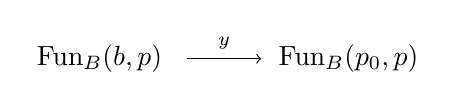
\begin{tikzpicture}[x=1.5em,y=1.5em]
  \node (L) at (0,0) {$\mathrm{Fun}_{B}(b,p)$};
  \node (R) at (6.0,0) {$\mathrm{Fun}_{B}(p_{0},p)$};
  \draw[->] (2.1,0) -- node[above]{$\scriptstyle y$} (3.9,0);
\end{tikzpicture}
\end{center}
\begin{center}
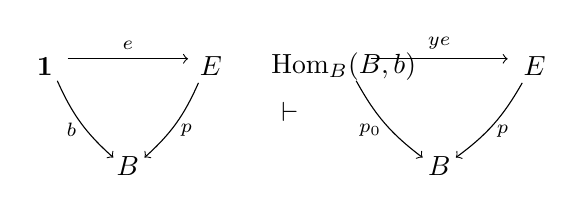
\begin{tikzpicture}[x=1.5em,y=1.5em]
  \begin{scope}[shift={(0,0)}]
  \node (o) at (0,1.1) {$\qcOne$};
  \node (E) at (4.0,1.1) {$E$};
  \node (B) at (2.0,-1.3) {$B$};
  \draw[->] (0.55,1.28) -- node[above]{$\scriptstyle e$} (3.45,1.28);
  \draw[->] (0.3,0.75) to[bend right=12] node[left,pos=0.6]{$\scriptstyle b$} (1.65,-1.1);
  \draw[->] (3.7,0.7) to[bend left=12] node[right,pos=0.6]{$\scriptstyle p$} (2.4,-1.1);
  \end{scope}
  \node at (5.9,0) {$\vdash$};
  \begin{scope}[shift={(7.2,0)}]
  \node (H) at (0,1.1) {$\mathrm{Hom}_{B}(B,b)$};
  \node (E) at (4.6,1.1) {$E$};
  \node (B) at (2.3,-1.3) {$B$};
  \draw[->] (0.65,1.28) -- node[above]{$\scriptstyle ye$} (3.95,1.28);
  \draw[->] (0.3,0.75) to[bend right=12] node[left,pos=0.6]{$\scriptstyle p_{0}$} (1.9,-1.1);
  \draw[->] (4.3,0.7) to[bend left=12] node[right,pos=0.6]{$\scriptstyle p$} (2.7,-1.1);
  \end{scope}
\end{tikzpicture}
\end{center}
上右 $\mathrm{Fun}_{B}(p_{0},p)$ 中的函子 $ye$ 定义了一个从 $p_{0}$ 到 $p$ 的
笛卡尔函子。
\end{lemma}

\begin{proof}
在\cref{prop:evaluation-right-adjoint}的证明中，右伴随由图
\eqref{eq:yoneda-transfer-cube} 定义为：见证\trTerminal{}元素之\trAdjunction{}%
的\trUnit{} $\eta$ 的 $q_{*}$-笛卡尔提升之定义域分量的一个分解。
此处 $q$ 是\trCartesianFibration{} $p$ 的一个\trPullback{}
\eqref{eq:representable-pullback}，故由命题 5.2.4，$y$ 同样可以描述为 $p_{0}\eta$
的 $p_{*}$-笛卡尔提升之定义域分量的分解，而后者等于右逗号锥
$\phi\colon p_{0}\Rightarrow b!$。
总之，函子 $y$ 定义如下：
\begin{center}
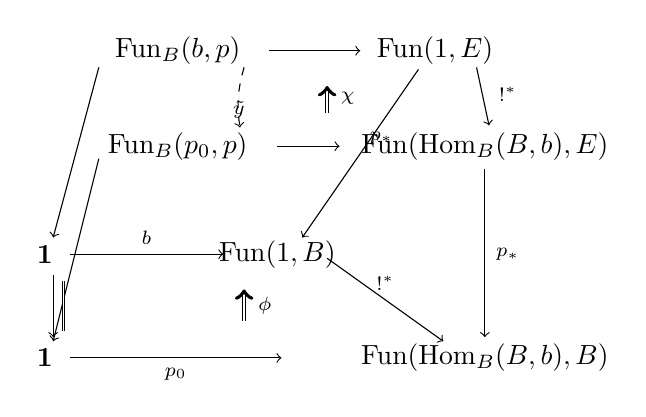
\begin{tikzpicture}[x=1.5em,y=1.5em]
  \node (BP) at (0,3.4) {$\mathrm{Fun}_{B}(b,p)$};
  \node (FE) at (6.2,3.4) {$\mathrm{Fun}(1,E)$};
  \node (PP) at (0,1.1) {$\mathrm{Fun}_{B}(p_{0},p)$};
  \node (HE) at (7.4,1.1) {$\mathrm{Fun}(\mathrm{Hom}_{B}(B,b),E)$};
  \node (o1) at (-3.2,-1.5) {$\qcOne$};
  \node (FB) at (2.4,-1.5) {$\mathrm{Fun}(1,B)$};
  \node (HB) at (7.4,-4.0) {$\mathrm{Fun}(\mathrm{Hom}_{B}(B,b),B)$};
  \node (o2) at (-3.2,-4.0) {$\qcOne$};
  \draw[->] (2.2,3.4) -- (4.4,3.4);
  \draw[->,dashed] (1.6,3.0) to[bend right=12] node[below,pos=0.4]{$\scriptstyle\tilde{y}$} (1.5,1.55);
  \draw[->] (7.2,3.0) -- (7.5,1.6);  \node at (7.95,2.35) {$\scriptstyle!^{*}$};
  \draw[double,->] (3.6,1.9) -- (3.6,2.55);
  \node at (4.1,2.25) {$\scriptstyle\chi$};
  \draw[->] (-1.9,3.0) -- (-3.0,-1.1);
  \draw[->] (-1.9,0.8) -- (-3.0,-3.6);
  \node at (1.1,2.9) {$\scriptstyle\llcorner$};
  \node at (1.0,0.6) {$\scriptstyle\llcorner$};
  \draw[->] (2.4,1.1) -- (3.9,1.1);
  \draw[->] (7.4,0.55) -- (7.4,-3.5);  \node at (7.95,-1.5) {$\scriptstyle p_{*}$};
  \draw[->] (5.8,2.95) -- (3.0,-1.1);  \node at (4.9,1.3) {$\scriptstyle p_{*}$};
  \draw[->] (-3.0,-2.0) -- (-3.0,-3.5);
  \draw[double] (-2.75,-2.15) -- (-2.75,-3.35);
  \draw[->] (-2.6,-1.5) -- node[above]{$\scriptstyle b$} (1.1,-1.5);
  \draw[->] (3.6,-1.6) -- (6.4,-3.6);  \node at (5.0,-2.2) {$\scriptstyle!^{*}$};
  \draw[double,->] (1.6,-3.1) -- (1.6,-2.35);
  \node at (2.1,-2.75) {$\scriptstyle\phi$};
  \draw[->] (-2.6,-4.0) -- node[below]{$\scriptstyle p_{0}$} (2.5,-4.0);
\end{tikzpicture}
\end{center}
于是，由引理 5.6.5，我们看到 $ye$ 是\trNaturalTransformation{}
$\phi\colon p_{0}\Rightarrow pe!$ 的 $p$-笛卡尔提升 $\chi e$ 的定义域分量
\begin{center}
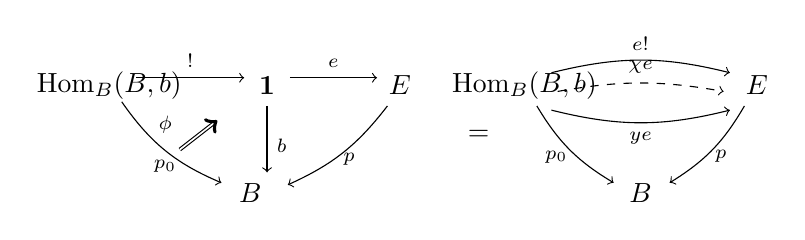
\begin{tikzpicture}[x=1.5em,y=1.5em]
  \begin{scope}[shift={(0,0)}]
  \node (H) at (0,1.2) {$\mathrm{Hom}_{B}(B,b)$};
  \node (o) at (3.8,1.2) {$\qcOne$};
  \node (E) at (7.0,1.2) {$E$};
  \node (B) at (3.4,-1.4) {$B$};
  \draw[->] (0.65,1.38) -- node[above]{$\scriptstyle !$} (3.25,1.38);
  \draw[->] (4.35,1.38) -- node[above]{$\scriptstyle e$} (6.45,1.38);
  \draw[->] (0.3,0.8) to[bend right=16] node[below,pos=0.5]{$\scriptstyle p_{0}$} (2.7,-1.15);
  \draw[->] (3.8,0.7) -- node[right,pos=0.6]{$\scriptstyle b$} (3.8,-0.9);
  \draw[->] (6.7,0.7) to[bend left=14] node[right,pos=0.6]{$\scriptstyle p$} (4.3,-1.2);
  \draw[double,->] (1.7,-0.35) -- (2.6,0.35);
  \node at (1.35,0.25) {$\scriptstyle\phi$};
  \end{scope}
  \node at (8.9,0) {$=$};
  \begin{scope}[shift={(10.0,0)}]
  \node (H) at (0,1.2) {$\mathrm{Hom}_{B}(B,b)$};
  \node (E) at (5.6,1.2) {$E$};
  \node (B) at (2.8,-1.4) {$B$};
  \draw[->] (0.65,1.5) to[bend left=14] node[above]{$\scriptstyle e!$} (4.95,1.5);
  \draw[->,dashed] (0.8,1.05) to[bend left=10] node[above,pos=0.5]{$\scriptstyle\chi e$} (4.8,1.05);
  \draw[->] (0.65,0.6) to[bend right=14] node[below,pos=0.5]{$\scriptstyle ye$} (4.95,0.6);
  \draw[->] (0.3,0.7) to[bend right=14] node[left,pos=0.6]{$\scriptstyle p_{0}$} (2.15,-1.15);
  \draw[->] (5.3,0.7) to[bend left=14] node[right,pos=0.6]{$\scriptstyle p$} (3.5,-1.15);
  \end{scope}
\end{tikzpicture}
\end{center}
由于 $p_{0}\colon\mathrm{Hom}_{B}(B,b)\twoheadrightarrow B$ 是离散的，余定义域为
$\mathrm{Hom}_{B}(B,b)$ 的每个\trNaturalTransformation{} $\psi$ 都是
$p_{0}$-\trCartesian，故为证 $ye$ 定义一个笛卡尔函子，我们必须证明 $ye\psi$ 是
$p$-\trCartesian。为此目的，考虑水平复合：
\begin{center}
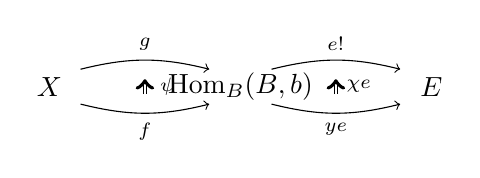
\begin{tikzpicture}[x=1.5em,y=1.5em]
  \node (X) at (0,0) {$X$};
  \node (H) at (4.6,0) {$\mathrm{Hom}_{B}(B,b)$};
  \node (E) at (9.2,0) {$E$};
  \draw[->] (0.75,0.42) to[bend left=14] node[above]{$\scriptstyle g$} (3.85,0.42);
  \draw[->] (5.35,0.42) to[bend left=14] node[above]{$\scriptstyle e!$} (8.45,0.42);
  \draw[->] (0.75,-0.42) to[bend right=14] node[below]{$\scriptstyle f$} (3.85,-0.42);
  \draw[->] (5.35,-0.42) to[bend right=14] node[below]{$\scriptstyle ye$} (8.45,-0.42);
  \draw[double,->] (2.3,-0.18) -- (2.3,0.18);
  \node at (2.85,0) {$\scriptstyle\psi$};
  \draw[double,->] (6.9,-0.18) -- (6.9,0.18);
  \node at (7.45,0) {$\scriptstyle\chi e$};
\end{tikzpicture}
\end{center}
由须化的自然性，$\chi g\cdot ye\psi=e!\psi\cdot\chi f$，而由于 $\qcOne$ 是%
\trTerminal{}∞-范畴，$e!\psi$ 是一个恒同。
于是，由 $p$-笛卡尔变换的左消去（见引理 5.1.5），$ye\psi$ 是 $p$-\trCartesian。
\end{proof}

为完成\cref{thm:yoneda-lemma}的证明，尚需论证这一受限\trAdjunction{}定义了一个%
\trAdjointEquivalence。

\begin{proof}[\cref{thm:yoneda-lemma}的证明]
由\cref{lem:cartesian-functor-right-adjoint}，\trAdjunction{}
\eqref{eq:yoneda-adjunction} 限制后定义了一个\trAdjunction
\begin{center}
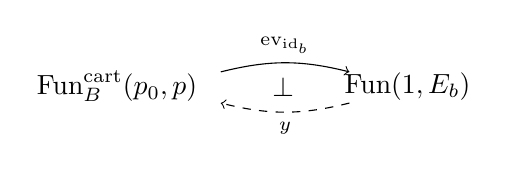
\begin{tikzpicture}[x=1.5em,y=1.5em]
  \node (L) at (0,0) {$\mathrm{Fun}_{B}^{\mathrm{cart}}(p_{0},p)$};
  \node (R) at (7.0,0) {$\mathrm{Fun}(1,E_{b})$};
  \draw[->] (2.5,0.35) to[bend left=14] node[above]{$\scriptstyle\mathrm{ev}_{\qcor{\mathrm{id}_{b}}}$} (5.6,0.35);
  \node at (4.0,0) {$\perp$};
  \draw[->,dashed] (5.6,-0.4) to[bend left=14] node[below]{$\scriptstyle y$} (2.5,-0.4);
\end{tikzpicture}
\end{center}
由于原本的\trAdjunction{} $!\dashv\qcor{\mathrm{id}_{b}}$ 的\trCounit{}是一个%
\trIsomorphism，且覆盖 2-函子在 2-胞腔上\trConservative，\cref{prop:evaluation-right-adjoint}
的\trAdjunction{}的\trCounit、从而还有受限\trAdjunction{}的\trCounit{}都是一个%
\trIsomorphism。与\cref{thm:discrete-yoneda-lemma}的证明中一样，我们通过论证
受限\trAdjunction{}的\trUnit{}也可逆来证明 $\mathrm{ev}_{\qcor{\mathrm{id}_{b}}}$
是一个\trEquivalence。由推论 1.1.22，只需逐元素地验证之，即证：以笛卡尔函子
\begin{center}
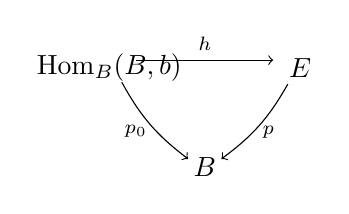
\begin{tikzpicture}[x=1.5em,y=1.5em]
  \node (H) at (0,1.1) {$\mathrm{Hom}_{B}(B,b)$};
  \node (E) at (4.6,1.1) {$E$};
  \node (B) at (2.3,-1.3) {$B$};
  \draw[->] (0.65,1.28) -- node[above]{$\scriptstyle h$} (3.95,1.28);
  \draw[->] (0.3,0.75) to[bend right=12] node[left,pos=0.6]{$\scriptstyle p_{0}$} (1.9,-1.1);
  \draw[->] (4.3,0.7) to[bend left=12] node[right,pos=0.6]{$\scriptstyle p$} (2.7,-1.1);
\end{tikzpicture}
\end{center}
为指标的\trUnit{}之分量是一个\trIsomorphism。

拆解\cref{prop:evaluation-right-adjoint}的证明：$\mathrm{ev}_{\qcor{\mathrm{id}_{b}}}\dashv y$
的\trUnit{} $\hat{\eta}$ 被定义为如下图表
\begin{center}
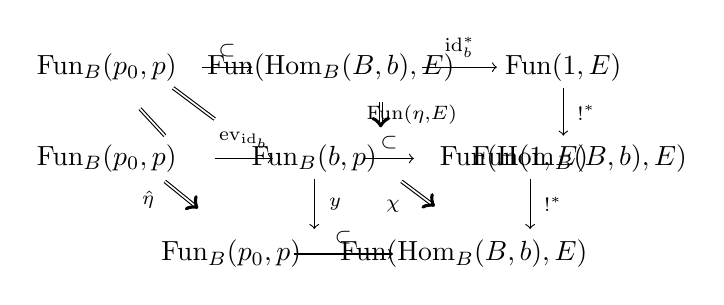
\begin{tikzpicture}[x=1.5em,y=1.5em]
  \node (P0) at (0,2.6) {$\mathrm{Fun}_{B}(p_{0},p)$};
  \node (HE1) at (5.4,2.6) {$\mathrm{Fun}(\mathrm{Hom}_{B}(B,b),E)$};
  \node (FE1) at (11.0,2.6) {$\mathrm{Fun}(1,E)$};
  \draw[->] (2.3,2.6) -- node[above]{$\scriptstyle\subset$} (3.5,2.6);
  \draw[->] (7.6,2.6) -- node[above]{$\scriptstyle\qcor{\mathrm{id}_{b}}^{*}$} (9.4,2.6);
  \draw[double] (1.6,2.1) -- (2.6,1.35);
  \draw[double,->] (6.6,1.75) -- (6.6,1.15);
  \node at (7.35,1.45) {$\scriptstyle\mathrm{Fun}(\eta,E)$};
  \draw[->] (11.0,2.1) -- (11.0,0.95);  \node at (11.55,1.5) {$\scriptstyle!^{*}$};
  \node (HE2) at (11.0,0.4) {$\mathrm{Fun}(\mathrm{Hom}_{B}(B,b),E)$};
  \draw[double] (0.8,1.6) -- (1.4,0.95);
  \node (P1) at (0,0.4) {$\mathrm{Fun}_{B}(p_{0},p)$};
  \node (BP) at (5.0,0.4) {$\mathrm{Fun}_{B}(b,p)$};
  \node (FE2) at (10.2,0.4) {$\mathrm{Fun}(1,E)$};
  \draw[->] (2.6,0.4) -- node[above]{$\scriptstyle\mathrm{ev}_{\qcor{\mathrm{id}_{b}}}$} (4.0,0.4);
  \draw[->] (6.2,0.4) -- node[above]{$\scriptstyle\subset$} (7.4,0.4);
  \draw[double,->] (1.4,-0.15) -- (2.2,-0.8);
  \node at (1.0,-0.6) {$\scriptstyle\hat{\eta}$};
  \draw[->] (5.0,-0.1) -- (5.0,-1.3);  \node at (5.5,-0.7) {$\scriptstyle y$};
  \draw[double,->] (7.1,-0.15) -- (7.9,-0.75);
  \node at (6.9,-0.75) {$\scriptstyle\chi$};
  \draw[->] (10.2,-0.1) -- (10.2,-1.3);  \node at (10.75,-0.7) {$\scriptstyle!^{*}$};
  \node (P2) at (3.0,-1.9) {$\mathrm{Fun}_{B}(p_{0},p)$};
  \node (HE3) at (8.6,-1.9) {$\mathrm{Fun}(\mathrm{Hom}_{B}(B,b),E)$};
  \draw[->] (4.5,-1.9) -- node[above]{$\scriptstyle\subset$} (6.9,-1.9);
\end{tikzpicture}
\end{center}
——即 $\mathrm{Fun}(\eta,E)$ 之限制穿过 $p_{*}$-笛卡尔提升 $\chi$ 的一个分解——
其中 $\eta$ 是\trAdjunction{} $!\dashv\qcor{\mathrm{id}_{b}}$ 的\trUnit。受限
2-胞腔 $\mathrm{Fun}(\eta,E)$ 在笛卡尔函子 $h$ 处的分量是 $h\eta$。由于
$p_{0}\colon\mathrm{Hom}_{B}(B,b)\twoheadrightarrow B$ 是一条\trDiscreteCartesianFibration，
任何余定义域为 $\mathrm{Hom}_{B}(B,b)$ 的 2-胞腔——例如 $\eta$——都是
$p_{0}$-\trCartesian；又因 $h$ 是一个笛卡尔函子，我们随即看到 $h\eta$ 是
$p$-\trCartesian。

由引理 5.6.6，$p_{*}$-笛卡尔胞腔 $\chi$ 的诸分量定义了环境∞-宇宙中的
$p$-笛卡尔\trNaturalTransformation。
由于 $\hat{\eta}$ 是余定义域为 $\mathrm{Fun}_{B}(p_{0},p)$ 的一个%
\trNaturalTransformation，其诸分量沿 $p$ 投影为恒同。这样，我们看到 $\hat{\eta}h$
是 $p$-笛卡尔变换 $h\eta$ 穿过「$\phi$ 在一个恒同之上的 $p$-笛卡尔提升」的分解，
而引理 5.1.12 证明 $\hat{\eta}h$ 是一个\trIsomorphism，正如所需。
\end{proof}

在∞-宇宙论中，我们有如下技巧可用：任何在一般∞-宇宙中被证明的结果——例如
\cref{thm:yoneda-lemma}——都可以应用于切片∞-宇宙。
这常可用来把关于一个∞-范畴之\trElement{}的结果扩充到该∞-范畴的广义元素
（例如见注 4.3.12）。
借助这一技巧，\cref{thm:yoneda-lemma}蕴含下述推广，它把元素 $b\colon\qcOne\to B$
换成广义元素 $b\colon X\to B$。

\begin{corollary}[广义 Yoneda 引理]\label{cor:generalized-yoneda-lemma}
对任意\trCartesianFibration{} $p\colon E\twoheadrightarrow B$ 与\trFunctor{}
$b\colon X\to B$，沿典范诱导的函子 $\qcor{\mathrm{id}_{b}}$ 作限制定义了拟范畴
之间的一个\trEquivalence：
\begin{center}
\begin{tikzpicture}[x=1.5em,y=1.5em]
  \begin{scope}[shift={(0,0)}]
  \node (X) at (0,1.1) {$X$};
  \node (H) at (4.6,1.1) {$\mathrm{Hom}_{B}(B,b)$};
  \node (B) at (2.3,-1.3) {$B$};
  \draw[->] (0.65,1.28) -- node[above]{$\scriptstyle\qcor{\mathrm{id}_{b}}$} (3.9,1.28);
  \draw[->] (0.3,0.75) to[bend right=12] node[left,pos=0.6]{$\scriptstyle b$} (1.9,-1.1);
  \draw[->] (4.3,0.7) to[bend left=12] node[right,pos=0.6]{$\scriptstyle p_{0}$} (2.7,-1.1);
  \end{scope}
  \node at (7.0,0) {$\rightsquigarrow$};
  \begin{scope}[shift={(8.4,0)}]
  \node (T) at (2.6,1.5) {$\mathrm{Fun}_{B}^{\mathrm{cart}}\bigl(\mathrm{Hom}_{B}(B,b)\xrightarrow{p_{0}}B,\,E\xrightarrow{p}B\bigr)$};
  \node (D) at (2.6,-1.3) {$\mathrm{Fun}_{B}\bigl(X\xrightarrow{b}B,\,E\xrightarrow{p}B\bigr)$};
  \draw[double,->] (2.6,0.9) -- (2.6,-0.55);
  \node at (4.35,0.2) {$\scriptstyle\mathrm{ev}_{\qcor{\mathrm{id}_{b}}}$};
  \end{scope}
\end{tikzpicture}
\end{center}
\end{corollary}

\cref{cor:generalized-yoneda-lemma}可以被解读为：为「笛卡尔纤维化与笛卡尔函子」
这一子范畴的包含函子定义了一个「左双伴随」，它把任意\trFunctor{}
$b\colon X\to B$ 反射入一条\trCartesianFibration{}
$p_{0}\colon\mathrm{Hom}_{B}(B,b)\twoheadrightarrow B$。

\begin{proof}
给定∞-宇宙 $\mathcal{K}$ 中的所陈数据。\cref{thm:yoneda-lemma}可应用于
$\mathcal{K}_{/X}$ 中的\trCartesianFibration{}
$p\times X\colon E\times X\twoheadrightarrow B\times X$ 与元素
$(b,X)\colon X\to B\times X$，从而定义一个\trEquivalence
\begin{center}
\begin{tikzpicture}[x=1.5em,y=1.5em]
  \node (t) at (0,1.5) {$\mathrm{Fun}_{B\times X}^{\mathrm{cart}}\bigl((p_{1},p_{0}),\,p\times X\bigr)\xrightarrow[\ \sim\ ]{\ \mathrm{ev}_{\qcor{\mathrm{id}_{(b,X)}}}\ }\mathrm{Fun}_{B\times X}\bigl((b,X),\,p\times X\bigr)$};
  \node (d) at (0,-1.3) {$\mathrm{Fun}_{B}^{\mathrm{cart}}\bigl(\mathrm{Hom}_{B}(B,b)\xrightarrow{p_{0}}B,\,E\xrightarrow{p}B\bigr)\xrightarrow[\ \sim\ ]{\ \mathrm{ev}_{\qcor{\mathrm{id}_{b}}}\ }\mathrm{Fun}_{B}\bigl(X\xrightarrow{b}B,\,E\xrightarrow{p}B\bigr)$};
  \draw[double] (-5.2,0.7) -- (-4.6,0.4);
  \draw[double] (4.6,0.7) -- (5.2,0.4);
\end{tikzpicture}
\end{center}
它在单纯伴随
\begin{center}
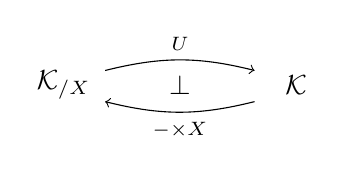
\begin{tikzpicture}[x=1.5em,y=1.5em]
  \node (L) at (0,0) {$\mathcal{K}_{/X}$};
  \node (R) at (5.6,0) {$\mathcal{K}$};
  \draw[->] (1.0,0.35) to[bend left=14] node[above]{$\scriptstyle U$} (4.6,0.35);
  \node at (2.8,0) {$\perp$};
  \draw[->] (4.6,-0.4) to[bend left=14] node[below]{$\scriptstyle-\times X$} (1.0,-0.4);
\end{tikzpicture}
\end{center}
之下转置为所述的\trEquivalence。
\end{proof}

尽管有其名，广义 Yoneda 引理并不是我们所需要的\trYonedaLemma{}的最一般形式。
这一结果的一个「双侧」版本出现在定理 7.3.2 中，其证明用的是同样的技巧：在一个
更为特异的∞-宇宙——即带固定底的余笛卡尔纤维化之宇宙——中应用
\cref{cor:generalized-yoneda-lemma}。
出于这个原因，我们邀请读者伴随我们走进一段间奏，在其中导出∞-宇宙的更多例子。

\subsection*{练习}

\begin{exercise}\label{ex:postcomposition-map}
设 $f\colon\qcOne\to\mathrm{Hom}_{A}(x,y)$ 是一个∞-范畴 $A$ 中一对元素之间的%
\trMappingSpace{}中的一个\trElement。请使用\cref{cor:mapping-space-evaluation}
之映射的逆\trEquivalence{}的显式描述，构造一个映射
\begin{center}
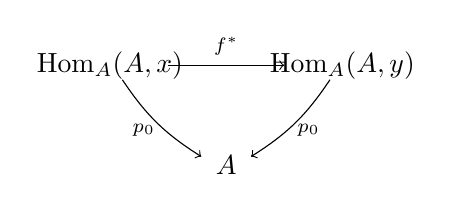
\begin{tikzpicture}[x=1.5em,y=1.5em]
  \node (Hx) at (0,1.1) {$\mathrm{Hom}_{A}(A,x)$};
  \node (Hy) at (5.6,1.1) {$\mathrm{Hom}_{A}(A,y)$};
  \node (A)  at (2.8,-1.3) {$A$};
  \draw[->] (1.4,1.1) -- node[above]{$\scriptstyle f^{*}$} (4.2,1.1);
  \draw[->] (0.3,0.75) to[bend right=12] node[left,pos=0.6]{$\scriptstyle p_{0}$} (2.2,-1.1);
  \draw[->] (5.3,0.75) to[bend left=12] node[right,pos=0.6]{$\scriptstyle p_{0}$} (3.4,-1.1);
\end{tikzpicture}
\end{center}
它表示由对 $f$ 作后复合所定义的「\trNaturalTransformation」。
\footnote{提示：这一构造是\cref{lem:cartesian-functor-right-adjoint}证明的前一半
所给出的构造的一个特例。}
\end{exercise}



